\documentclass[11pt,a4paper]{article}

\usepackage[utf8]{inputenc}
\usepackage{graphics}
\usepackage{url}
\usepackage{amssymb} % Simbolos matematicos
\usepackage{graphicx}
\usepackage{graphics}

\newcommand{\finejercicio}{
  \begin{footnotesize}
    [Al terminar el ejercicio es recomendable hacer \texttt{commit} de los ficheros modificados]
  \end{footnotesize}
}

\newcommand{\finpractica}{
  \begin{footnotesize}
    [Al terminar la práctica, realiza un \texttt{push} para sincronizar tu repositorio GitLab]
  \end{footnotesize}
}

%\renewcommand{\finejercicio}{}
%\renewcommand{\finpractica}{}


\ProcessOptions

\begin{document}


\title{Práctica 5 - Sesión SIP}
\author{Protocolos para la Transmisión de Audio y Vídeo en Internet}
\date{Versión 10.1 - 30.11.2020}


\maketitle

Nota: Esta práctica se puede entregar para su evaluación como parte de la nota de prácticas. Para las instrucciones de entrega, mira al final del documento. 

\section{Introducción}

El protocolo de iniciación de sesión (SIP) es un protocolo que se limita solamente al establecimiento y control de una sesión (RFC 3550). Los detalles del intercambio de datos, como por ejemplo la codificación o decodificación del audio/vídeo, no son controlados por SIP sino que se llevan a cabo por otros protocolos (por ejemplo, RTP). Los principales objetivos de SIP son:

\begin{itemize}
  \item SIP permite el establecimiento de una localización de usuario (o sea, traducir de un nombre de usuario a su dirección de red actual)
  \item SIP provee funcionalidad para la negociación de las características de una sesión, de manera que los participantes en una sesión pueden consensuar características soportadas por todos ellos.
  \item SIP es un mecanismo para la gestión de llamadas, por ejemplo para añadir, eliminar o transferir participantes
  \item SIP permite la modificación de características de la sesión durante su transcurso.
\end{itemize}

\section{Objetivos de la práctica}

\begin{enumerate}
  \item Conocer el protocolo SIP y otros protocolos utilizados en una sesión con clientes SIP (como \texttt{Ekiga} o \texttt{linphone}).
  \item Profundizar en el uso de \texttt{Wireshark}: análisis, captura y filtrado.
\end{enumerate}

\section{Conocimientos previos necesarios}

\begin{itemize}
  \item Nociones de SIP y RTP (las de clase de teoría)
  \item Funcionamiento de \texttt{Wireshark}.
\end{itemize}

Tiempo estimado (para un alumno medio): 8 horas


\section{Ejercicios}

\begin{enumerate}

\subsection*{Creación de repositorio para la práctica}

  \item Con el navegador, dirígete al repositorio \texttt{ptavi-p5} en la cuenta de la asignatura en GitLab\footnote{\url{http://gitlab.etsit.urjc.es/ptavi/ptavi-p5}} y realiza un \texttt{fork}, de manera que consigas tener una copia del repositorio en tu cuenta de GitLab. Clona el repositorio que acabas de crear a local para poder editar los archivos. Trabaja a partir de ahora en ese repositorio, sincronizando los cambios que vayas realizando.

  Como tarde al final de la práctica, deberás realizar un \texttt{push} para subir tus cambios a tu repositorio en GitLab. En esta práctica, al contrario que con las demás, se recomienda hacer frecuentes \texttt{commits}, pero el \texttt{push} al final.


\subsection*{Análisis de una sesión SIP}

Se ha capturado una sesión SIP con el cliene SIP Ekiga (archivo \texttt{sip.cap.gz}), que se puede abrir con \texttt{Wireshark}\footnote{Desde la shell: \texttt{\$ wireshark sip.cap.gz} - recuerda que puedes utilizar el tabulador en la shell para autocompletar.}. Se pide rellenar las cuestiones que se plantean en este guión en el fichero \texttt{p5.txt} que encontrarás también en el repositorio. 

  \item Observa que las tramas capturadas corresponden a una sesión SIP con \texttt{Ekiga}, un cliente de VoIP para \texttt{GNOME}. Responde a las siguientes cuestiones:
  \begin{itemize}
    \item ¿Cuántos paquetes componen la captura?
    \item ¿Cuánto tiempo dura la captura?
    \item ¿Qué IP tiene la máquina donde se ha efectuado la captura? ¿Se trata de una IP pública o de una IP privada? ¿Por qué lo sabes?
  \end{itemize}

  \item Antes de analizar las tramas, mira las estadísticas generales que aparecen en el menú de \texttt{Statistics}. En el apartado de jerarquía de protocolos (\texttt{Protocol Hierarchy}) se puede ver el porcentaje del tráfico correspondiente al protocolo TCP y UDP.
  \begin{itemize}
    \item ¿Cuál de los dos es mayor? ¿Tiene esto sentido si estamos hablando de una aplicación que transmite en tiempo real? 
    \item ¿Qué otros protocolos podemos ver en la jerarquía de protocolos? ¿Cuales crees que son señal y cuales ruido?
  \end{itemize}

  \item Observa por encima el flujo de tramas en el menú de \texttt{Statistics} en \texttt{IO Graphs}. La captura que estamos viendo incluye desde la inicialización (registro) de la aplicación hasta su finalización, con una llamada entremedias. 
  \begin{itemize}
    \item Filtra por \texttt{sip} para conocer cuándo se envían paquetes SIP. ¿En qué segundos tienen lugar esos envíos?
    \item Y los paquetes con RTP, ¿cuándo se envían?
  \end{itemize}

  \finejercicio

  \item Analiza las dos primeras tramas de la captura. 
  \begin{itemize}
    \item ¿Qué servicio es el utilizado en estas tramas?
    \item ¿Cuál es la dirección IP del servidor de nombres del ordenador que ha lanzado Ekiga? 
    \item ¿Qué dirección IP (de \texttt{ekiga.net}) devuelve el servicio de nombres? 
  \end{itemize}

  \item A continuación, hay más de una docena de tramas TCP/HTTP.
  \begin{itemize}
    \item ¿Podrías decir la URL que se está pidiendo? 
    \item ¿Qué \texttt{user agent} (UA) la está pidiendo? 
    \item ¿Qué devuelve el servidor?
    \item Si lanzamos el navegador web, por ejemplo, \texttt{Mozilla Firefox}, y vamos a la misma URL, ¿qué recibimos? ¿Qué es, entonces, lo que está respondiendo el servidor? 
  \end{itemize}

  \item Hasta la trama 45 se puede observar una secuencia de tramas del protocolo STUN.
  \begin{itemize}
    \item ¿Por qué se hace uso de este protocolo?
    \item ¿Podrías decir si estamos tras un \texttt{NAT} o no?
  \end{itemize}

  \item La trama 46 es la primera trama SIP. En un entorno como el de Internet, lo habitual es desconocer la dirección IP de la otra parte al realizar una llamada. Por eso, todo usuario registra su localización en un servidor \texttt{Registrar}. El \texttt{Registrar} guarda información sobre los usuarios en un servidor de localización que puede ser utilizado para localizar usuarios.
  \begin{itemize}
    \item ¿Qué dirección IP tiene el servidor \texttt{Registrar}?
    \item ¿A qué puerto (del servidor \texttt{Registrar}) se envían los paquetes SIP?
    \item ¿Qué método SIP utiliza el UA para registrarse?
    \item Además de \texttt{REGISTER}, ¿podrías decir qué instrucciones SIP entiende el UA?
  \end{itemize}

  \finejercicio

  \item Fijémonos en las tramas siguientes a la número 46:
  \begin{itemize}
    \item ¿Se registra con éxito en el primer intento? 
    \item ¿Cómo sabemos si el registro se ha realizado correctamente o no? 
    \item ¿Podrías identificar las diferencias entre el primer intento y el segundo de registro? (fíjate en el tamaño de los paquetes y mira a qué se debe el cambio)
    \item ¿Cuánto es el valor del tiempo de expiración de la sesión? Indica las unidades.
  \end{itemize}


  \item Una vez registrados, podemos efectuar una llamada. Vamos a probar con el servicio de eco de Ekiga que nos permite comprobar si nos hemos conectado correctamente. El servicio de eco tiene la dirección \texttt{sip:500@ekiga.net}. Veamos el \texttt{INVITE} de cerca.
  \begin{itemize}
    \item ¿Puede verse el nombre del que efectúa la llamada, así como su dirección SIP?
    \item ¿Qué es lo que contiene el cuerpo de la trama? ¿En qué formato/protocolo está?
    \item ¿Tiene éxito el primer intento? ¿Cómo lo sabes?
    \item ¿En qué se diferencia el segundo \texttt{INVITE} más abajo del primero? ¿A qué crees que se debe esto?
  \end{itemize}

  \item Una vez conectado, estudia el intercambio de tramas. 
  \begin{itemize}
    \item ¿Qué protocolo(s) se utiliza(n)? ¿Para qué sirven estos protocolos?
    \item ¿Cuál es el tamaño de paquete de los mismos?
    \item ¿Se utilizan bits de \texttt{padding}?
    \item ¿Cuál es la periodicidad de los paquetes (en origen; nota que la captura es en destino)?
    \item ¿Cuántos bits/segundo se envían?
  \end{itemize}

  \finejercicio

  \item Vamos a ver más a fondo el intercambio RTP. En \texttt{Telephony} hay una opción RTP. Empecemos mirando los flujos RTP.
  \begin{itemize}
    \item ¿Cuántos flujos hay? ¿por qué?
    \item ¿Cuántos paquetes se pierden?
    \item ¿Cuál es el valor máximo del delta? ¿Y qué es lo que significa el valor de \texttt{delta}?
    \item ¿Cuáles son los valores de \texttt{jitter} (medio y máximo)? ¿Qué quiere decir eso? ¿Crees que estamos ante una conversación de calidad?
  \end{itemize}

  \item Elige un paquete RTP de audio. Analiza el flujo de audio en \texttt{Telephony -> RTP -> Stream Analysis}.
  \begin{itemize}
    \item ¿Cuánto valen el \texttt{delta} y el \texttt{jitter} para el primer paquete que ha llegado?
    \item ¿Podemos saber si éste es el primer paquete que nos han enviado?
    \item Los valores de \texttt{jitter} son menores de 10ms hasta un paquete dado. ¿Cuál?
    \item ¿A qué se debe el cambio tan brusco del \texttt{jitter}?
    \item ¿Es comparable el cambio en el valor de \texttt{jitter} con el del \texttt{delta}? ¿Cual es más grande? 
  \end{itemize}

  \item En \texttt{Telephony} selecciona el menú \texttt{VoIP calls}. Verás que se lista la llamada de voz IP capturada en una ventana emergente. Selecciona esa llamada y pulsa el botón \texttt{Play Streams}.
  \begin{itemize}
    \item ¿Cuánto dura la conversación?
    \item ¿Cuáles son sus SSRC? ¿Por qué hay varios SSRCs? ¿Hay CSRCs?
  \end{itemize}


  \item Identifica la trama donde se finaliza la conversación. 
  \begin{itemize}
    \item ¿Qué método SIP se utiliza?
    \item ¿En qué trama(s)?
    \item ¿Por qué crees que se envía varias veces?
  \end{itemize}

  \item Finalmente, se cierra la aplicación de VozIP.
  \begin{itemize}
    \item ¿Por qué aparece una instrucción SIP del tipo \texttt{REGISTER}?
    \item ¿En qué trama sucede esto?
    \item ¿En qué se diferencia con la instrucción que se utilizó con anterioridad (al principio de la sesión)?
  \end{itemize}

  \finejercicio

\subsection*{Captura de una sesión SIP}


  \item Dirígete a la web de Linphone\footnote{\url{https://www.linphone.org/freesip/home}} con el navegador y créate una cuenta SIP.  Recibirás un correo electrónico de confirmación en la dirección que has indicado al registrarte (mira en tu carpeta de \emph{spam} si no es así).
  
  \item Lanza \texttt{linphone}, y configúralo con los datos de la cuenta que te acabas de crear. Para ello, puedes ir al menú ``Opciones'' y seleccionar ``Preferencias'' (o pulsando ``Ctrl+P'').

  \item Verás una ventana similar a la que se muestra en la figura~\ref{fig:preferencias}. En la parte superior, verás tus credenciales del laboratorio. Necesitamos crear una \emph{cuenta proxy}, para lo que pulsaremos sobre el botón de ``+ Añadir'' en la parte derecha.

% Comprueba que estás conectado (En la barra al final de la ventana podrás ver ``Registrado'').
%Tendrás que rellenar los campos de manera similar a lo que se puede ver en la imagen a continuación (recuerda poner tu nombre de usuario en lugar de ``grex'').
\begin{center}
\begin{figure}[h!]
\center
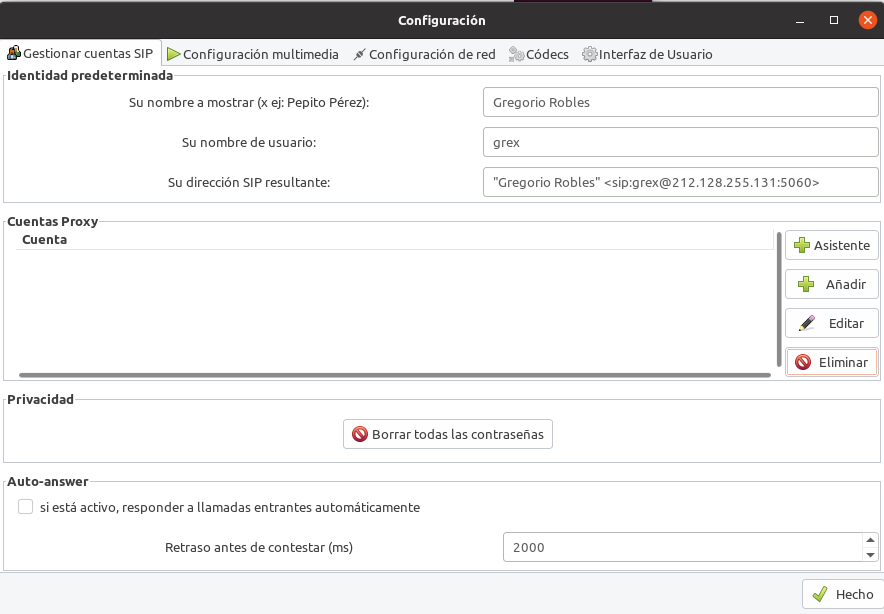
\includegraphics[width=0.5\textwidth]{figs/preferencias.png}
\caption{Ventana de preferencias de Linphone.}
\label{fig:preferencias}
\end{figure}
\end{center}
  
   \item Rellena con tus datos en el menú de la ventana emergente, similar a la figura~\ref{fig:configuracion}. Si introduces tus datos de manera correcta, te pedirá la contraseña de tu cuenta SIP en linphone.org que hemos creado en un apartado anterior.

\begin{center}
\begin{figure}[h!]
\center
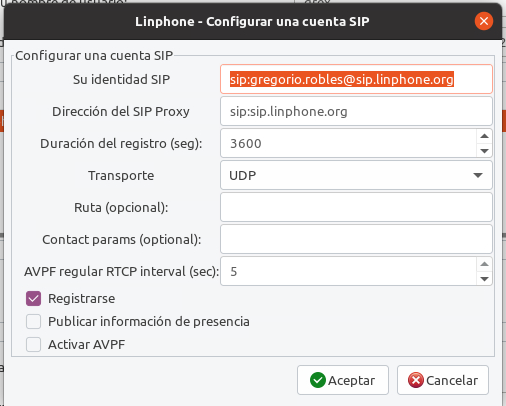
\includegraphics[width=0.5\textwidth]{figs/configuracion.png}
\caption{Configuración de cuenta SIP proxy en Linphone.}
\label{fig:configuracion}
\end{figure}
\end{center}

  \item Cierra completamente linphone. Captura una sesión SIP de una conversación con el número SIP \texttt{sip:music@sip.iptel.org}. Recuerda que has de comenzar a capturar tramas antes de arrancar linphone para ver todo el proceso\footnote{Puedes \emph{matar} linphone desde la línea de \texttt{shell} buscando el identificador del proceso con \$ ps aux y terminándolo con \$ kill -9 \emph{pid}, donde \emph{pid} es el identificador del proceso.}.

  \item Observa las diferencias en el inicio de la conversación entre el entorno del laboratorio y el del ejercicio anterior\footnote{Si estás utilizando tu portátil en vez de una máquina del laboratorio, ten en cuenta que la captura puede ser diferente, porque con el portátil estarás conectado a la red \emph{wifi}, mientras que los ordenadores de los laboratorios lo están a una LAN.}:
  \begin{itemize}
    \item ¿Se utilizan DNS y STUN? ¿Por qué?
    \item ¿Son diferentes el registro y la descripción de la sesión?
  \end{itemize}

  \item Identifica las diferencias existentes entre esta conversación y la conversación anterior:
  \begin{itemize}
    \item ¿Cuántos flujos tenemos?
    \item ¿Cuál es su periodicidad?
    \item ¿Cuánto es el valor máximo del delta y los valores medios y máximo del jitter?
    \item ¿Podrías reproducir la conversación desde \texttt{Wireshark}? ¿Cómo? Comprueba que poniendo un valor demasiado pequeño para el \texttt{buffer} de \texttt{jitter}, la conversación puede no tener la calidad necesaria.
    \item ¿Sabrías decir qué tipo de servicio ofrece \texttt{sip:music@iptel.org}?
  \end{itemize}

  \finejercicio

  \item Filtra por los paquetes SIP de la captura y guarda {\bf únicamente} los paquetes SIP como \texttt{p5.pcapng}. Abre el fichero guardado para cerciorarte de que lo has hecho bien. Deberás añadirlo al repositorio.

  \finejercicio
  
  \finpractica

\end{enumerate}

\section{Fecha y modo de entrega}

La entrega de práctica se deberá hacer antes del miércoles 2 de diciembre de 2020 a las 23:59. Para entonces, se debe: 

\begin{itemize}
  \item Tener un repositorio git en GitLab con:
  \begin{enumerate}
    \item Un archivo de texto con los comentarios a los ejercicios en \texttt{p5.txt}.
    \item Un archivo con una captura filtrada en \texttt{p5.pcapng}.
    \item Un test de \texttt{Moodle} rellenado sobre la práctica 5. Este test tendrá preguntas relacionadas con los ejercicios que se han realizado y tiene un tiempo de realización de 20 minutos.
    \item 4 ficheros adicionales (además de \texttt{.git}): \texttt{README.md}, \texttt{LICENSE}, \texttt{check-p5.py} y \texttt{.gitignore}.
  \end{enumerate}
\end{itemize}

Se ha de tener en cuenta las siguientes consideraciones:
\begin{itemize}
  \item Se valorará que al menos haya diez \texttt{commits} realizados en al menos dos días diferentes
  \item Se valorará que la captura esté bien filtrada y sólo contenga los paquetes que se indican en el guión.
\end{itemize}

Se puede comprobar la correcta entrega de la práctica utilizando el programa \texttt{check-p5.py}. Este programa se ejecuta desde la línea de comandos de la siguiente manera:
\begin{verbatim}
	$ python check-p5.py login
\end{verbatim}


donde \texttt{login} es tu nombre de usuario en los laboratorios docentes. El programa comprueba que se han entregado los ficheros que se solicitan (y sólo esos). 


%\vspace{1cm}

%\footnotesize{Para el final: Si a estas alturas todavía tienes ganas, puedes indicar en el Moodle el tiempo que te ha llevado realizar esta práctica. Esto te lleva menos de un minuto y nos sirve a los profesores para hacernos una idea del esfuerzo que os lleva. ¡Gracias!}

\end{document}
